\subsection{ECU's Externas}

Para poder probar cualquier cosa del gateway primero se necesitaban un par de componentes externos que interactuaran con este mismo, como se muestra en la figura \ref{} del datasheet del gateway.

\begin{figure}[!htb]
 \centering
 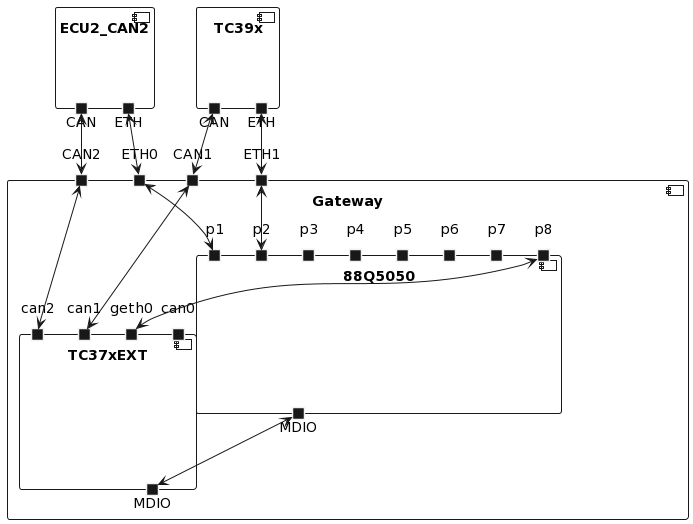
\includegraphics[width=\textwidth]{img/GWConnectionsDiagram.png}
 \caption{Gateway Connections Diagram}
 \label{fig:connections-diagram}
\end{figure}

\subsection{First Demo}
En el primer demo para hacer la prise en main de AUTOSAR habia un ejemplo el cual debia funcionar con el programa CANoe. Se intento replicar el comportamiento del CANoe haciendole ingenieria inversa a los codigos. Se encontro el CanId necesario para que el ECU recibiera el frame CAN pero al parecer esto sigue un protocolo mas preciso por parte del programa del demo (CANoe). Decidimos dejarlo aqui porque eso no era productivo para el proyecto pero se aprendio muchisimo de autosar y de la forma en como esta estructurado su stack de comunicacion.

%\begin{verbatim}
%/* Appl/GenData/CanIf_Lcfg.c L279 */
%CONST(CanIf_RxPduConfigType, CANIF_CONST) CanIf_RxPduConfig[8] = {  /* PRQA S 1514, 1533 */  /* MD_CSL_ObjectOnlyAccessedOnce */
%    /*Index    RxPduCanId  RxPduMask  UpperPduId                                  RxIndicationFctListIdx   RxPduDlc   MsgType                      
%  { /* 0 */    0x0400u  ,  0x643Fu  , CanNmConf_CanNmRxPdu_CAN_5f8bc0cc_Rx      , 1u               ,       8u         , CANIF_MSG_TYPE_CAN       },
%  { /* 1 */    0x0614u  ,  0x07FFu  , CanTpConf_CanTpRxNPdu_CanTpRxNPdu_e872022a, 2u               ,       8u         , CANIF_MSG_TYPE_NO_FD_CAN },
%  { /* 2 */    0x0610u  ,  0x07FFu  , CanTpConf_CanTpRxNPdu_CanTpRxNPdu_29945216, 2u               ,       8u         , CANIF_MSG_TYPE_NO_FD_CAN },
%  { /* 3 */    0x0501u  ,  0x07FFu  , PduRConf_PduRSrcPdu_PduRSrcPdu_7a86d966   , 3u               ,      64u         , CANIF_MSG_TYPE_CAN       },
%  { /* 4 */    0x0310u  ,  0x07FFu  , PduRConf_PduRSrcPdu_PduRSrcPdu_37e6280b   , 3u               ,       4u         , CANIF_MSG_TYPE_CAN       },
%  { /* 5 */    0x0210u  ,  0x07FFu  , PduRConf_PduRSrcPdu_PduRSrcPdu_9e00b2d3   , 3u               ,       1u         , CANIF_MSG_TYPE_CAN       },
%  { /* 6 */    0x0120u  ,  0x07FFu  , PduRConf_PduRSrcPdu_PduRSrcPdu_01c8980f   , 3u               ,       8u         , CANIF_MSG_TYPE_CAN       },
%  { /* 7 */    0x0110u  ,  0x07FFu  , PduRConf_PduRSrcPdu_PduRSrcPdu_b1d1dd8a   , 3u               ,       6u         , CANIF_MSG_TYPE_CAN       } 
%};
%\end{verbatim}

Primero habia un demo en el que habia un sistema de autosar bastante mas simple para el cual tuvimos que hacer varias cosas antes de arrancar, como hackearle el flexray y eso. Luego creamos un modelo en python que enviara datos por CAN. Despues de leer el stack de comunicacion de Autosar me di cuenta que habian varias cosillas que no tenian logica y al parecer el sw wstaba mal planteado. 

\subsection{Gateway}

Un gateway es un nodo de una red que se comunica con una red exterior, usualmente mas grande. Las ventajas de este gateway es que permite conectar varios protocolos de comunicacion como el Fr, CAN, LIN o ETH, para complementar ECU's que no necesariamente esten programadas para utilizarlos. 

Este gateway en si mismo es una ECU programable con el sistema operativo MICROSAR Classic en el cual podemos preprocesar datos antes de comunicarnos con un protocolo exterior. 

Ademas de esto, este gateway cuenta con un switch ethernet securise que soporta un ancho de banda y velocidades muy altas. Esto permite, por ejemplo, a un sistema de inteligencia artifial de conduccion acceder a una camara de 4k a traves de ethernet (por el ancho de banda grande que este tipo de media necesita) procesar datos y hacer una bien su trabajo, pero al tiempo puede pedir datos o enviar a otra ECU por LIN o CAN sin tener el protocolo fisico integrado. Tambien se pueden recibir muchos datos de internet como estado del trafico o datos de navegacion en tiempo real sin saturar protocolos de comunicacion como el LIN o Fr que tienen muchisimo menos ancho de banda.


\subsection{TC37xEXT}
Al comienzo del proyecto empezamos usando el microcontrolador AURIX TC37x \cite{aurix.tc37x} pero luego leyendo el datasheet del Gateway nos dimos cuenta que en realidad se estaba usando el TC37xEXT \cite{aurix.tc37e} el cual es una version con mas modulos disponibles, entre ellos un modulo CAN y un modulo GETH extras los cuales serian utiles en nuestro proyecto. Otras diferencias se encuentran en la tabla \ref{tab:tc37x_delta}.


% Table generated by Excel2LaTeX from sheet 'Sheet1'
\begin{table}[htbp]
  \centering
    \begin{tabular}{|r||l|l|}
	\hline
	\multirow{2}{*}{Module} & \multicolumn{2}{c|}{Aurix}\\
	\cline{2-3}
	& TC37x & TC37xEXT \\
	\hline \hline
	    RAM & TRAM (cached, non-cached) & EMEM (cached, non-cached) \\
	    \hline
	    CAN interfaces & 2 & 3 \\
	    \hline
	    Camera Interface & not present & CIF \\
	    \hline
	    Gigabit Ethernet Interface & 1 & 2 \\
	    \hline
	    SD interface & not present & present \\
	    \hline
	    eMMC interface & not present & present \\
	    \hline
	\hline
    \end{tabular}
  \caption{TC37x Vs TC37xEXT}
  \label{tab:tc37x_delta}
\end{table}


Para modelisar los microcontroladores se utiliza python2, tomamos los modelos de cada modulo (memorias, mcmcan, cpus, etc) y los unimos a un bus con su respectiva start address y luego lo compilamos. Al final agregamos el nuevo microcontrolador al toolbox ya creado para poder tener todo bien clean.

El siguiente paso fue testear el microcontrolador. Para programar en estos microcontroladores se usa BIFACES, un compilador especial para estas CPU's. Para testear las memorias se escribieron datos y se leyeron luego. Para el modulo CAN y GETH se testearon sus memorias RAM y se enviaron un par de mensajes hacia una ECU externa  y se verificaron. Todo salio bien y pudimos avanzar con el proyecto.

\subsection{Switch Marvell 88Q5050}

Para que el demo arranque nosotros el sw hace ciertas verificaciones de sus componentes como buses de datos funcionales y verifica el correcto comportamiento de ciertos componentes. En este contexto, el switch marvell 88Q5050 juega una papel muy importante en este proceso. El microcontrolador tiene una secuencia muy precisa para verificar el correcto comportamiento del switch, incluyendo leer y escribir registros por el BUS MDIO y descargar todos los registros del switch para luego usarlos. La secuencia de inicializacion esta detallada en el anexo \ref{anexe:switch-init}. Si se enceuntran errores en esta secuencia de inicializacion el sistema operativo no va a inicar los puertos de comunicacion ethernet y por tanto los demos del gateway no van a funcionar de la mejor manera.

Para modelar el switch se utilizo systemC. Se modelo el Switch con base a la informacion fournie por parte del fabricante y se siguio con el proyecto.

\subsection{Use Case 1}

En la figura \ref{fig:connections-diagram} podemos ver que se tienen

\begin{figure}[!htb]
 \centering
 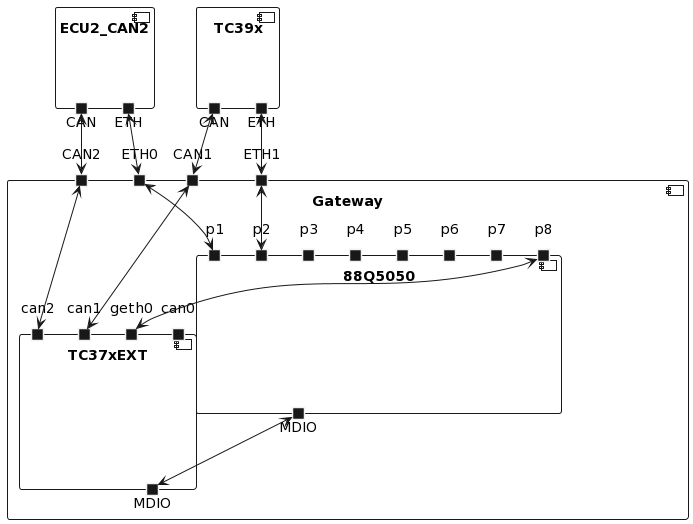
\includegraphics[width=\textwidth]{img/GWConnectionsDiagram.png}
 \caption{Gateway Connections Diagram}
 \label{fig:connections-diagram}
\end{figure}


%Ya con el microcontrolador correcto podemos pasar al demo precargado en microsar tiene 2 USe cases en los que primero se envia algo por CAN y se le hace un forward por eth y viceversa.
%Segun la documentacion del gateway, este gateway esta conectado de la forma mostrada en la figura \ref{fig:connections-diagram}. 

\begin{figure}[!htb]
 \centering
 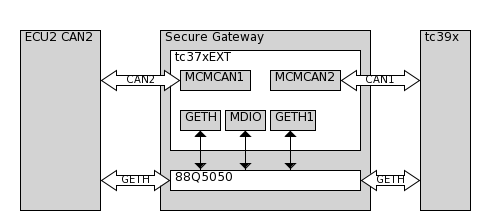
\includegraphics[width=\textwidth]{img/gateway_block_diagram.png}
 \caption{Gateway Block diagram}
 \label{fig:block diagram}
\end{figure}

Tonces lo primero que habia que hacer era tener algun tipo de componente que envie datos por el bus can y por ethernet para que sean recibidos por el 
Tonces lo primero que habia que hacer era leer el stack de comunicaciones de autosar y saber lo que el 
\subsection{Use Case 1}
En este Gateway hay una cierta cantidad de componentes que hay que modelar porque el software intenta comunicarse con ellos. Cogi el modelo que habia desarrollado en el caso anterior y le puse funcionalidades de Ethernet y de LIN (para un posterior uso) y lo conecte con el AURIX como se muestra en la figura \ref{fig:connections-diagram}


Al comienzo no nos planteamos necesario modelar el switch pero luego nos dimos cuenta que el AURIX se intenta comunicar con el y sin sus respuestas no hay nada que funcione. Aqui les pones un UML de la secuencia de verificacion del switch. Resulta que los switches tienen un modo que se llama RMU que significa Remote management Unit y eso entra en una categoria que se llama Distributed Switch Architecture que permite que puedas controlar un switch con una cpu externa. En este caso se usa en la secuencia de inicializacion para tener acceso a los registros del switch. Para esto se ajusta el modo RMU desde los pines del MDIO y luego se mandan datos por ethernet en el puerto 8 (IMPORTANTE QUE SEA SOLO EL PUERTO 8) con un Tag especial de protocolo SNAP (SubNetwork A Protocol) (en este punto nos toco agregar support para los codigos SNAP en el modelo del microcontrolador) y luego se envia un arespuesta siguiendo el protocolo de Marvell. hasta aqui lo llevo yo el dia de hoy.

Luego muestras que envias un dato desde CAN con el id que es y que no funcionaba porque patata

\subsection{Use Case 2}

Ni idea que voy a poner aqui.
